\documentclass[../MA_Thesis.tex]{subfiles}
\renewcommand{\baselinestretch}{1.5} 
\usepackage{hyperref}
\usepackage{csquotes}

\begin{document}
\subsection*{Participants}
Participants were recruited through Amazon Mechanical Turk (MTurk) and compensated \$2.00 for the online experiment that takes around 15 to 20 minutes (at an approximate rate of \$7.50 per hour). 

An a priori power analysis was conducted using G*Power version 3.1.9.6 (\cite{faul_gpower_2007}) to determine the minimum required sample size for detecting differences in arousal levels between mood conditions. Based on data from \textcite{sugawara_effect_2021}, which compared high-arousal and low-arousal positive emotions in a thought–action repertoire task using film clips for mood induction, the reported effect size was d = 1.42 for arousal ratings, a large effect according to \textcite{cohen_power_1992}'s criteria. Given a significance threshold of $\alpha = .05$ and power = .95, the minimum required sample size for a two-tailed independent samples t-test is N = 12 per group. 

This power analysis was conducted to ensure that the mood induction procedure effectively differentiates high-arousal and low-arousal states and that any observed effects on creativity are attributable to mood rather than sample size limitations. The finalized sample size for the online experiment was N = 90 (30 per group), exceeding the required minimum and providing sufficient statistical power to detect mood-related differences in arousal and subsequent cognitive performance. Participants were required to be physically present in the United States, as verified by their IP address.

% Think about specifics of exclusion here
Participants who [] were excluded from the analysis, resulting in a final sample of [N] participants (Mage = X, SD = X; X males, X females, X non-binary/other).

This study was approved by the Institutional Review Board (IRB) of the University of Chicago, and all participants provided their informed consent before beginning the experiment.

\subsection*{Experiment Design}
To test the proposed flexibility pathway linking positive activating mood with the originality aspect of creativity, this study employed a between-subjects design with three experimental conditions for mood induction: 1) high-arousal positive mood, 2) low-arousal positive mood, and 3) neutral control condition. We then used the incomplete shape drawing task (\cite{barbot_dynamics_2018}) to capture the flexibility and originality aspects of creativity. By integrating these methodological approaches, the study aimed to empirically validate the hypothesized mediating role of flexibility in the relationship between mood and creative output.

Our online experiment was implemented using jsPsych (\cite{leeuw_jspsych_2023}), a JavaScript framework designed to conduct behavioral experiments on web browsers. The website was structured into three main sections (see Figure \ref{fig: Experiment Web Page Design} for the overall structure of the experiment): (1) mood induction, (2) incomplete shape drawing tasks, and (3) survey data collection.

\begin{figure}
    \centering
    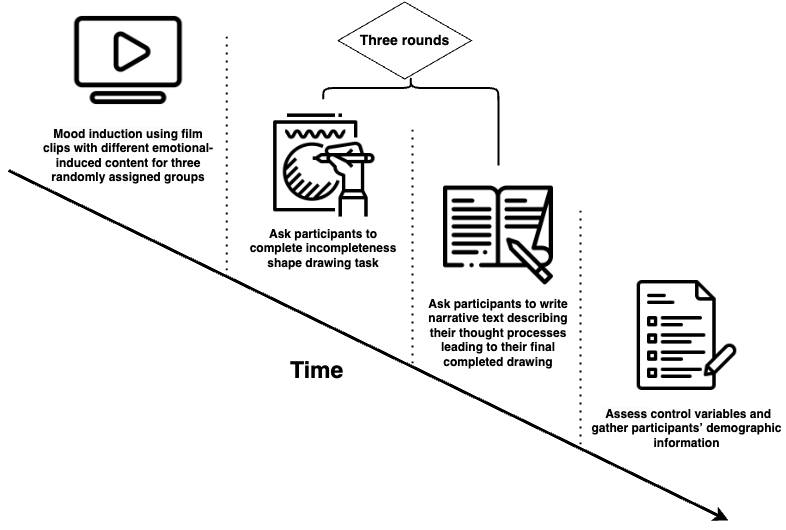
\includegraphics[width=0.7\linewidth, keepaspectratio]{drawio/Experiment Timeline.png}
    \caption{Experiment Web Page Design}
    \label{fig: Experiment Web Page Design}
\end{figure}

\subsubsection*{Mood Induction}
After completing informed consent, participants underwent mood induction by watching film clips, which has been shown to be an effective mood induction technique to engage visual and auditory modalities and simulate real-life emotional situations (\cite{coan_handbook_2007}; \cite{fernandez-aguilar_how_2019}; \cite{siedlecka_experimental_2019}). Participants were randomly assigned to one of the three mood induction conditions (high arousal positive, low arousal positive, or neutral). 

To induce positive high-arousal and negative-arousal mood states, we used two film clips validated by \textcite{wensveen_push_2002} that tap into positive valence mood at the polar ends of the arousal continuum within the Circumplex Model of Mood (\cite{feldman_variations_1995}). These film clips were validated through the Mood Induction Procedure (MIP; \cite{lench_discrete_2011}), where participants rated their valence and arousal levels using the Self-Assessment Manikin (SAM; \cite{bradley_affect_1999}), a graphic figure representing the valence and arousal elements in mood states. Specifically, for high-arousal positive mood, we used a 2:55-minute clip from \textit{Blues Brothers} as in \cite{wensveen_push_2002}'s study. This scene features an energetic gospel performance, with James Brown and the Rev. James Cleveland Choir singing \textit{The Old Landmark}. The combination of lively music, dynamic movement, and expressive enthusiasm evokes an elevated state of excitement and joy, representing high-arousal positive affect. Meanwhile, for low-arousal positive mood, we chose a 2:38-minute clip from \textit{Easy Rider}. This scene depicts the protagonists riding motorcycles along a tranquil desert highway at sunset, accompanied by \textit{The Weight} by The Band. Smooth pacing, warm visual tones, and a soothing soundtrack induce a relaxed and peaceful emotional state, representing a low arousal positive affect. Finally, for the neutral control group, we followed \textcite{maryam_fakhrhosseini_affectemotion_2017}'s and \textcite{siedlecka_experimental_2019}'s approach, in which neutral affect is typically induced using low-arousal, emotionally neutral visual stimuli (e.g., nature documentaries and weather news). In this study, we chose a 1:56-minute UK morning weather forecast from Met Office. 

Before viewing the video clips, participants received the instruction to immerse themselves in the clip as they would when watching a movie in a cinema, without needing to memorize any details from the clips they would be watching. This way, the framing effects on induced moods could be minimized, as opposed to using more directive prompts like ``Let yourself experience your emotions fully.'' To assess the effectiveness of mood induction, participants rated their valence and arousal levels using SAM (\cite{bradley_affect_1999}). Valence ranged from -4 (very negative) to +4 (very positive), and arousal ranged from 1 (low) to 9 (high). 

\subsubsection*{Incomplete Shape Drawing Tasks}
After mood induction, participants completed the Incomplete Shape Drawing Task (\cite{barbot_dynamics_2018}), where participants encountered an incomplete shape and were encouraged to fully engage their imagination, take their time, and produce a drawing that was as creative as possible. Each participant was presented with three qualitatively distinct incomplete shapes, selected from three different stimulus groups and presented in a randomized order. This multi-trial approach aligns with \textcite{barbot_dynamics_2018}, facilitating an in-depth exploration of the dynamics of creative thinking and allowing researchers to examine within-subject variation in flexibility and originality. 

The task was implemented using a web-based drawing interface developed with the sketchpad plugin of jsPsych (\cite{leeuw_jspsych_2023}). This interactive interface provided participants with essential drawing tools, including options for undoing, redoing, and clearing strokes, ensuring an intuitive user experience. In addition to capturing the final drawing, the system recorded x, y coordinates and the timing of mouse movements throughout the drawing process. These data were stored in a JSON-like structure using base64 encoding for subsequent computational analysis (\cite{bainbridge_tutorial_2022}).

Following each drawing session, participants were prompted to give a label for each completed drawing. They were then asked to provide a detailed narrative describing their step-by-step thought process behind their completed drawing. Specifically, they reflected on their initial impressions of the incomplete shape—what first came to mind upon seeing it and whether it reminded them of anything specific. They were encouraged to discuss whether multiple ideas were considered before settling on a final concept and to elaborate on how their idea evolved during the drawing process, including any triggers for conceptual shifts. Meanwhile, they were also encouraged to identify the theme or category their drawing fit into, such as nature, technology, people, animals, or abstract concepts, and discussed whether any new themes emerged as they worked. This narrative was designed to capture participants' forming of associative connections of different semantic categories, tapping into the flexibility aspect of creativity. 

\subsubsection*{Survey Data Collection}
Once participants had finished mood induction and incomplete drawing tasks, they completed several survey questions related to the control variables and demographics. Including these control measures is crucial to improving causal inference by accounting for individual differences that could otherwise confound the relationship between mood and creativity.

Participants first completed several questionnaires that assess control variables, including trait affectivity (measured by the Positive and Negative Affect Schedule; \cite{watson_development_1988}) to control for baseline emotional tendencies that could impact mood-induction effects. Furthermore, openness to experiences (measured by the Ten Item Personality Measure; \cite{gosling_very_2003}) was included, as prior research suggests that individuals high in openness are more likely to have higher intrinsic motivation and creative process engagement, both of which enhance creativity (\cite{tan_openness_2019}). To further account for variations in cognitive adaptability, participants completed the Cognitive Flexibility Scale (\cite{martin_new_1995}), which assesses one's trait-level ability to change perspectives and adapt to new information, both critical for creative ideation (\cite{lin_how_2014}; \cite{muller_concentrative_2016}). Additionally, self-rated artistic skill was included to examine whether prior artistic experience influences task performance, ensuring that creativity differences are not solely attributable to skill level.

After completing these control measures, participants provided demographic information, including age, gender, race, and education level, allowing for an exploration of potential demographic influences on creativity and mood responses. These demographic variables also help contextualize the findings and ensure that the results are generalizable across diverse populations. 

%%%%%%%%%%%%%%%%%%%%%%%%%%%%%%%%%%%%%%%%%%%%%%
\subsection*{Creativity Assessment}
\subsubsection*{Measuring the Flexibility Aspect of Creativity}
According to \textcite{nijstad_dual_2010}'s dual pathway to creativity model, the flexibility aspect of creativity centers on employing wide-ranging and comprehensive cognitive categories to form associations. In the context of the incompleteness shape drawing task, flexibility specifically refers to the ability of participants to explore a wide range of qualitatively distinct creative solutions through two complementary operationalizations: 1) real-time, observable stroke decisions during the drawing process and 2) post-hoc reflective narratives about their thought processes.

The real-time, observable stroke decisions focus on participants’ ability to dynamically generate diverse and innovative strokes as they navigate the spatial and conceptual possibilities of the incomplete shape. Each stroke reflects an immediate decision, offering insights into how participants engage with qualitatively distinct creative solutions (both in terms of starting position and trajectory) for each stroke and make creative choices in real-time. On the other hand, the post-hoc narrative aspect emphasizes how participants recollect and articulate their cognitive processes, including their ability to connect disparate ideas, integrate themes, and explain their conceptual shifts. These narratives capture the depth and diversity of associative thinking, offering a window into how participants structure and evaluate their creative decisions retrospectively.

Together, these operationalizations provide a nuanced understanding of flexibility, capturing both the dynamic, moment-to-moment exploration of ideas and the reflective integration of conceptual categories, offering a more comprehensive view of creative ideation.

\paragraph*{Real-Time Stroke Decisions}
To gain insight into the flexibility aspect of creativity via real-time stroke decisions during the drawing process, we used the Compositional Stroke Embedding (CoSE) model that predicts the starting position and trajectory of the next stroke using the Gaussian Mixture Model (GMM). That GMM is able to forecast strokes with both varying degrees of uncertainty in its prediction and between-component (potential stroke) distances matches our operational definition of flexibility. Specifically, a more creatively flexible individual will not only consider a broader array of potential next strokes, but will also remain open to choosing other paths that are qualitatively distinct from each other in their choice space during their creative processes.

To quantify these characteristics, we utilized two key measures derived from the GMM: \textbf{entropy} and \textbf{Bhattacharyya distance} (see Appendix \ref{appendix: entropy} and Appendix \ref{appendix: bhattacharyya distance} for details of their formulas). Entropy captures the degree of uncertainty in the GMM predictions, reflecting the breadth of possible next strokes available to participants at a given moment. A higher entropy value indicates a wider range of creative possibilities, reflecting an individual's ability to explore diverse options. On the other hand, Bhattacharyya distance is a metric of similarity that ranges from 0 to $\infty$, where a smaller value indicates a higher degree of similarity (or overlap) between the two distributions, and a higher value suggests greater divergence. It is particularly useful in the context of GMM for assessing overlap and separation between different clusters (\cite{alangari_intrinsically_2023}). In the context of incomplete drawing task, Bhattacharyya distance measures the divergence between potential next strokes (GMM components), providing insight into the distinctiveness of the paths being considered. A greater distance between components suggests a more varied and inclusive exploration of qualitatively distinct possibilities.

To map the dynamic changes in these two measures throughout the drawing process to the flexibility pathway of creativity, we selected two summary metrics that capture distinct facets of creative exploration: the average values of the measures and the proportion of inflection points. These metrics reflect the ability to not only consider a broader array of potential next strokes but also remain open to exploring alternative paths that are qualitatively distinct within the possibility space. Together, they provide insight into how participants navigate and engage with the total possibility space of next strokes during their creative processes. The average values and proportion of inflection points highlight both the sustained breadth of exploration and the dynamic shifts in strategy that characterize flexible creative behavior. These metrics enable a more comprehensive and nuanced analysis of how participants navigate the possibility space of next strokes during the drawing task.

The \textbf{average values} of entropy and Bhattacharyya distance serve as cumulative indicators of a participant’s overall creative breadth and divergence across the entire drawing task. High average entropy reflects a consistent ability to maintain a wide range of potential next strokes, indicating that the participant explores a large portion of the possibility space throughout the task. This measure captures the participant’s sustained openness to generating diverse options and avoiding early fixation on a single creative trajectory. Similarly, a high average Bhattacharyya distance suggests that participants consistently consider strokes that are qualitatively distinct from each other, emphasizing their ability to incorporate varied and unconventional approaches into their creative process. By summarizing the overall level of exploration and divergence, the average values provide a bird’s-eye view of a participant’s capacity to engage with the task’s inherent creative possibilities and remain broadly flexible over time.

The \textbf{proportion of inflection points}, in contrast, delves deeper into the moments of dynamic change within the creative process. Inflection points—defined as significant shifts in the trends of entropy or Bhattacharyya distance—represent critical junctures where participants reconsider their trajectory or diverge from their current path. A higher proportion of inflection points suggests that participants frequently engage in deliberate transitions between different creative strategies, reflecting their ability to pivot dynamically within the possibility space. These moments of change are particularly important in understanding flexibility because they indicate a willingness to disrupt the status quo, reframe the problem, and explore new directions. This adaptability, captured through the proportion of inflection points, complements the broader patterns revealed by the average values and provides a richer understanding of how participants dynamically engage with alternative possibilities throughout their creative process. In this study, we used the Pruned Exact Linear Time (PELT) algorithm (\cite{dorcas_wambui_power_2015}) that utilizes \textit{ruptures} Python library (\cite{truong_selective_2020}) to identify the inflection point(s).

\paragraph*{Post-Hoc Narrative}
Complementing real-time, observable stroke decisions throughout the incomplete drawing task, this study also relied on the verbal description of the participants about their thought processes behind their completed drawings to examine the diversity of ideas/concepts they connect during creative ideation processes. As one type of observation offering data on individuals' cognitive processes (\cite{ericsson_verbal_2003}), verbal report could serve as a window into people's thought processes and the dynamics of creative thinking by requiring the organization and expression of ideas, reflecting the cognitive processes involved in structuring and connecting these ideas. As individuals construct stories, they engage in memory retrieval, association, and synthesis, which are key components of creative thinking. Narratives unfold over time, mirroring the dynamic nature of creative thought, allowing researchers to observe how ideas evolve, merge, and diverge.

Specifically, this study will utilize Divergent Semantic Integration (DSI; see Appendix \ref{appendix: DSI}) for its formula) to measure the diversity of concepts participants connected to complete incomplete shapes, inferred through their narrative about how they have approached and completed the drawings (\cite{johnson_divergent_2022}). DSI echoes \textcite{kaufman_cambridge_2010}'s call for interdisciplinary approaches to measure creativity by integrating \textcite{mednick_associative_1962}'s associative theory with distributional semantics theory in the linguistics field to assess how narratives integrate divergent ideas. On the one hand, DSI captures the essence of creativity featuring forming associations between disparate concepts in memory. On the other hand, DSI capitalizes on the theory of distributional semantics, which allows a computational understanding of semantics (word meanings) in a salable manner. Specifically, distributional semantics is based on the Distributional Hypothesis, which posits that words with similar meanings occur in similar contexts (\cite{lenci_distributional_2008}). By analyzing word co-occurrence in large text corpora, this approach creates vector-based representations of words in a high-dimensional space, and the proximity of these vectors reflects semantic similarity, allowing distributional semantics to capture word meanings based on usage patterns (\cite{boleda_distributional_2020}). Together, individuals with higher flexibility aspect of creativity would navigate further in his/her concept space to connect more distinct concepts, which predicts a higher DSI.

\subsubsection*{Measuring the Originality Aspect of Creativity}
To measure \textit{originality} aspect of creatvity, this study will refer to the pre-trained AuDrA model and implementation code provided on \textcite{patterson_audra_2023}'s \href{https://osf.io/kqn9v/}{open-access repository}. In an attempt to overcome the limitations of subjective creativity scoring, including labor cost and subjectivity, these authors joined the movement to capitalize on machine learning to automatically assess creativity (e.g., \cite{acar_applying_2023}; \cite{beaty_automating_2021}). Targeting at the tablet-based drawing task under \textcite{barbot_dynamics_2018}'s MTCI framework, AuDrA extends the (mere) fluency measurement via reaction time data in the original task by developing an automated method to assess the originality of the sketches.

As a modified ResNet architecture that allows continuous prediction of creativity scores, AuDra model was trained using over 13,000 sketches rated for creativity by nearly 60 human raters across four datasets. It used a supervised learning approach, utilizing the human-provided ratings as feedback to optimize its predictive accuracy for the specific task of visual creativity assessment. AuDrA demonstrated a high correlation with human creativity ratings in new drawings on the same task. In addition, AuDrA performance in predicting creativity scores surpassed the correlations between level of elaboration (ink on the page) in drawings and human creativity ratings, suggesting that AuDrA is sensitive to features of drawings beyond simple complexity or elaboration. 

Adopting AuDrA is suitable for my proposed research for three reasons. First, the drawing task I plan to implement is the same as the one AuDrA was trained on. Second, it allows automated originality assessment (with evidence of good model performance), which counts as a more feasible option in terms of my dispensable resources. Third, that AuDrA measures the \textit{originality} aspect of creativity complements the adoption of CoSE that captures the \textit{flexibility} aspect of creativity. Together, these two models enable me to examine the complete (hypothetical) flexibility pathway from positive activating mood to the originality aspect of creativity.

\subsection*{Statistical Analysis}

To examine the hypothesized flexibility pathway linking positive activating mood to originality in creativity, we employ mediation analysis (\cite{mackinnon_mediation_2007}) within the framework of the dual pathway to creativity model (\cite{de_dreu_hedonic_2008}). Specifically, we test whether the effect of mood induction (independent variable, IV) on the originality aspect of creativity (dependent variable, DV) is mediated by the flexibility aspect of creativity (mediator, M), as assessed through multiple quantitative measures.

Mediation analysis is well-suited for this study as it allows for a systematic examination of whether the flexibility aspect of creativity serves as a cognitive mechanism linking mood induction to originality. First, it enables an empirical test of the dual pathway to creativity model, which posits that mood influences originality through cognitive flexibility, by assessing whether flexibility statistically mediates this relationship. Second, mediation analysis allows for the decomposition of total effects into direct and indirect effects, distinguishing whether positive activating mood enhances originality directly or indirectly via flexibility. This distinction is crucial in determining whether flexibility is a necessary cognitive pathway in mood-induced creative enhancement.

Following best practices in mediation analysis (\cite{homburg_mediation_2022}), we leveraged randomized experimental design to strengthen causal inference. The random assignment of participants to mood conditions helps prevent any observed relationships between mood and creativity from being confounded by pre-existing differences in cognitive abilities. Furthermore, we controlled affectivity, openness to experiences, trait-level cognitive flexibility, and self-rated artistic skill, reducing potential alternative explanations for observed effects.

\subsubsection*{Mediation Model Specification}
The independent variable (IV) comprises three mood conditions: Happiness (\(D1\)), Calmness (\(D2\)), and Neutral (reference category). Following recommendations for categorical predictors in mediation models \cite{hayes_statistical_2014}, we dummy-coded the mood conditions to compare each experimental group against the neutral condition. The dependent variable (\(Y\))—originality in creativity—is measured using the AuDrA model, which predicts creativity ratings based on visual output.

The mediator (\(M\))—cognitive flexibility—is operationalized through multiple quantitative measures reflecting different facets of the flexibility pathway. Specifically, entropy of GMM predictions captures uncertainty in stroke selection, Bhattacharyya distance between GMM components reflects the divergence among predicted strokes, and Divergent Semantic Integration (DSI) measures conceptual flexibility in narrative descriptions. For entropy and Bhattacharyya distance, they are further decomposed into two components: the average value, which represents the overall level of exploration across the drawing process, and the proportion of inflection points, which captures fluctuations in flexibility, indicating shifts between exploratory and convergent thinking. Given that these mediators may independently contribute to originality, we estimate separate mediation models for each.

For each mediator (\(M_k\)), we estimate the following \textbf{mediator model}:
\begin{equation*}
    M_k = \alpha_0 + \alpha_1 D1 + \alpha_2 D2 + \alpha_3 X + \epsilon_{M_k}
\end{equation*}
where \( M_k \) represents each mediator: \( M_1a \) = Average entropy, \( M_1b \) = Proportion of entropy inflection points, \( M_2a \) = Average Bhattacharyya distance, \( M_2b \) = Proportion of Bhattacharyya distance inflection points, \( M_3 \) = DSI; \( \alpha_0 \) is the intercept; \( \alpha_1 \) and \( \alpha_2 \) are coefficients for the mood conditions; \( X \) is the vector of control variables; \( \epsilon_{M_k} \) is the error term.

Meanwhile, for each mediator, the \textbf{outcome model} is similarly expressed as:
\begin{equation*}
    Y = \beta_0 + \beta_1 D1 + \beta_2 D2 + \beta_3^k M_k + \beta_4 X + \epsilon_Y
\end{equation*}
where \( Y \) is originality in creativity; \( \beta_0 \) is the intercept; \( \beta_1 \) and \( \beta_2 \) capture the direct effects of mood condition; \( \beta_3^k \) represents the effect of each mediator on originality; \( \beta_4 X \) accounts for control variables; \( \epsilon_Y \) is the error term.

\subsubsection*{Testing Direct, Indirect, and Total Effects}
To evaluate the hypothesized flexibility pathway, we systematically tested \textbf{direct effects}, \textbf{indirect effects}, and \textbf{total effects} in the aforementioned mediation model, offering insights into which aspects of flexibility serve as potential mechanisms for creative originality.

The direct effects, captured by \( \beta_1 \) (Happiness) and \( \beta_2 \) (Calmness), measure the extent to which mood conditions influence originality (\(Y\)) independently of cognitive flexibility. A significant direct effect suggests that mood itself contributes to originality beyond its impact on flexibility. If these coefficients remain significant while mediation is present, it indicates \textit{partial mediation}, meaning mood enhances originality both directly and through flexibility.

The key test of mediation involves the indirect effects, quantified as:
\begin{equation*}
    \alpha_k \times \beta_3^k
\end{equation*}
for each mediator (\(M_k\)), where \( \alpha_k \) represents the effect of mood on the flexibility measure, and \( \beta_3^k \) represents the effect of the flexibility measure on originality. A significant indirect effect suggests that cognitive flexibility partially or fully explains the link between mood and creativity. Following \textcite{preacher_asymptotic_2008}'s approach, we used bootstrapping with 5,000 resamples to estimate the confidence interval (CI) for indirect effects, providing a more robust inference of mediation pathways. A mediation effect is significant if the bootstrap CI does not include zero.

The total effect captures the overall impact of mood on originality, combining both direct and indirect pathways:
\begin{equation*}
    \beta_1 + (\alpha_k \times \beta_3^k) \quad \text{(for Happiness)}
\end{equation*}
\begin{equation*}
    \beta_2 + (\alpha_k \times \beta_3^k) \quad \text{(for Calmness)}
\end{equation*}
where each term represents the contribution of a single mediator tested in separate models.

A significant total effect confirms that mood induction influences originality, regardless of whether the effect is primarily direct, indirect, or a combination of both. If the direct effect is insignificant while the indirect effect remains significant, it suggests full mediation, suggesting that cognitive flexibility fully accounts for mood-induced changes in originality.

\end{document}